\section{Zielsetzung}
Bei diesen Experimenten soll das Ablenkverhalten eines Elektronenstrahls in einem
elektrischen und einem magnetischen Feld untersucht werden.
Zudem soll mittels Ablenkung in einem magnetischen Feld die spezifische Elekronenladung
sowie das Magnetfeld der Erde am Ort der Messung bestimmt werden.
\section{Theorie}
\subsection{Kathodenstrahlröhre}
Da freie Elektronen üblicherweise mit Luftmolekülen wechselwirken würden, lässt sich
dieses Experiment nur im Hochvakuum durchführen, was in diesem Fall durch eine weitgehend
evakuierte Kathodenstrahlröhre realisiert wird, welche in Abbildung \ref{fig:rohr} schematisch dargestellt
ist.
\begin{figure}[H]
  \centering
  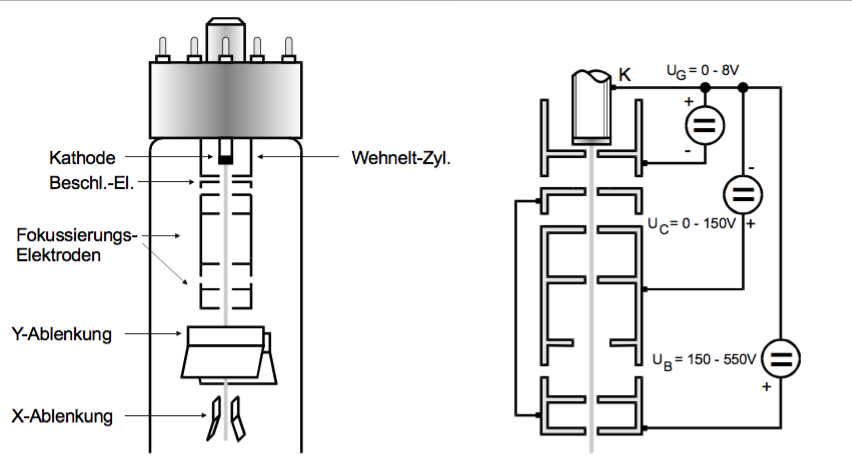
\includegraphics[height=5cm]{Rohr.png}
  \caption{Aufbau einer Kathodenstrahlröhre \cite{skript1}.}
  \label{fig:rohr}
\end{figure}
In dieser treten zunächst Elektronen aus der sogenannten Kathode aus, was auf dem glühelektrischen
Effekt beruht. Die Kathode ist dabei von einem  Wehnelt-Zylinder umgeben, über welchen
sich durch das negative Potential bezüglich der Kathode die Intensität des Strahls regulieren lässt.

Besitzen die Elektronen genug Energie um die Potentialdifferenz zu
überwinden, treten diese durch eine Bohrung aus dem Zylinder aus und werden durch eine
Beschleunigungsspannung $ U_B $ auf eine Geschwindigkeit von
\begin{equation}
  v_z = \sqrt{\frac{2 \text{e}_0 \cdot U_B }{\text{m}_0}}
  \label{eqn:geschwindigkeit}
\end{equation}
beschleunigt, welche sich aus dem Energiesatz ergibt. Hierbei bezeichnet $\text{e}_0$
die Elementarladung und $\text{m}_0$ die Elektronenmasse.
Anschließend wird der Elektronenstrahl durch eine elektronische Linse mittels inhomogene
Felder fokussiert.
Daraufhin durchläuft er zwei elektrisch aufladbare Plattenpaare, welche den Strahl aus
seiner ursprünglichen Bahn ablenken und somit den Auftreffpunkt verschieben.
Dieser Auftreffpunkt wird mittels Lichtquantenemission auf dem Schirm sichtbar gemacht.

\subsection{Ablenkung im elektrischen Feld}
Das Prinzip der Ablenkung des Elektronenstrahls ist in Abbildung \ref{fig:abl1}
dargestellt.
\begin{figure}[H]
  \centering
  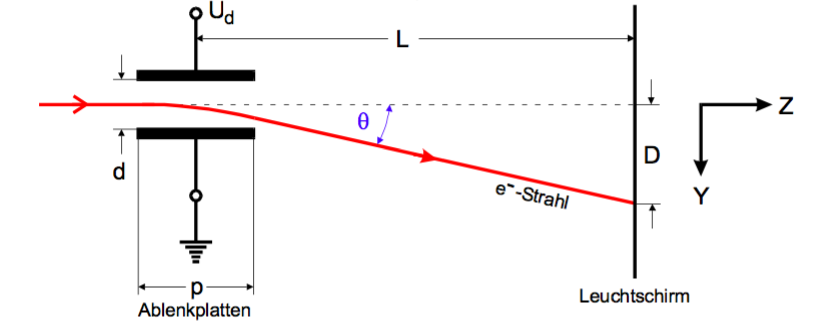
\includegraphics[height=5cm]{Ablenkung.png}
  \caption{Ablenkung des Elektronenstrahls im elektrischen Feld \cite{skript1}.}
  \label{fig:abl1}
\end{figure}
Durch die Relation d<<p lässt sich das Elektrische Feld zwischen den Platten zu
\begin{equation}
  E = \frac{U_d}{d}
  \label{eqn:efeld}
\end{equation}
nähern, wobei das Feld außerhalb der Platten prakisch Null ist.
Durch die komponentenweise Betrachtung der Geschwindigkeit sowie der Betrachtung
des Winkels der Ablenkung lässt sich durch Umformungen folgende Gleichung für
die Verschiebung D herleiten:
\begin{equation}
   D = \frac{\text{L} \cdot \text{p} \cdot U_d}{2\text{d} \cdot U_B}
   \label{eqn:verschiebung}
\end{equation}
Es lässt sich somit eine Proportionalität von D und $U_d$ festellen.

\subsection{Kathodenstrahl-Oszillograph}
Ein weiterer Verwendungszweck der Kathodenstrahlröhre ist der Kathodenstrahl-Oszillograph.
Hierzu wird an eines der beiden ablenkenden Plattenpaare eine Sägezahnspannung angeschlossen
und an das senkrecht dazu stehende Plattenpaar die zu untersuchende Wechselspannung.
Dadurch lässt sich der zeitliche Verlauf der zu untersuchenden Spannung auf
dem Leuchtschirm optisch darstellen, sobald die beiden Frequenzen in einem
geeigneten rationalen Verhältniss zueinander stehen.

\subsection{Ablenkung im magnetischen Feld}
In einem magnetischen Feld wirkt nur auf relativ zu dem Feld bewegten Ladungen die sogenannte
Lorentzkraft
\begin{equation}
  \vec{F}_L = q \cdot \vec{v} \times \vec{B} \: ,
  \label{eqn:lorentz}
\end{equation}
welche stets senkrecht auf der Bewegungsrichtung der Ladungen sowie dem magnetischen
Feld steht und in diesem Experiment für die Ablenkung des Elektronenstrahls sorgt.
Aus der Bedingung des Gleichgewichts von Lorentzkraft und Zentrifugalkraft in Verbindung
mit dem Energiesatz folgt, das der Strahl hierdurch einen Kreis mit Radius
\begin{equation}
  r = \frac{\text{m}_0 \cdot \text{v}_0}{\text{m}_0} \cdot B
  \label{eqn:radius}
\end{equation}
beschreibt.
Die konstante Geschwindigkeit der Elektronen $\text{v}_0$ lässt sich in mithilfe
des Energiesatzes zu
\begin{equation}
  \text{v}_0 = \sqrt{2 U_B \cdot \text{e}_0 / \text{m}_0}
  \label{eqn:v0}
\end{equation}
bestimmen.

Die tätsichlich messbare Verschiebung des Auftreffpunkts auf dem Leuchtschirm
ergibt sich somit durch die Gleichungen \ref{eqn:radius} und \ref{eqn:v0} und die
geometrischen Beziehungen, welche in Abbildung \ref{fig:magnet} dargestellt sind zu
\begin{equation}
   \frac{D}{D^2 + L^2} = \frac{1}{\sqrt{8 U_B}}\sqrt{\frac{\text{e}_0}{\text{m}_0}}\cdot B \: .
   \label{eqn:magnet}
\end{equation}

\begin{figure}[H]
  \centering
  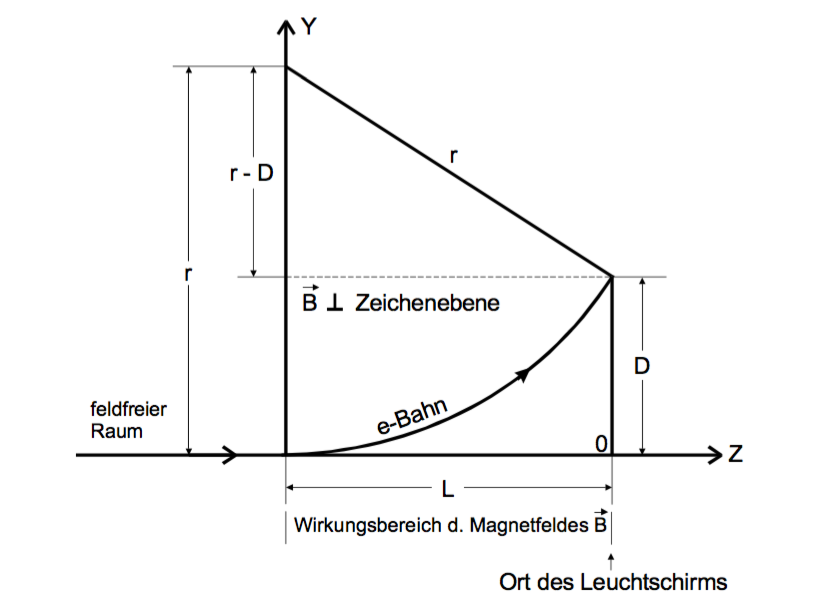
\includegraphics[height=5cm]{Magnet.png}
  \caption{Ablenkung des Elektronenstrahls im magnetischen Feld \cite{skript2}.}
  \label{fig:magnet}
\end{figure}
Hieraus kann man zum Beispiel die spezifische Ladung $ \frac{{\text{e}_0}}{{\text{m}_0}} $
der Elektronen bestimmen.
